% The flowchart tricks were taken from this article:
% https://www.overleaf.com/learn/latex/LaTeX_Graphics_using_TikZ:_A_Tutorial_for_Beginners_(Part_3)%E2%80%94Creating_Flowcharts
\documentclass[tikz]{standalone}
%\usepackage{fontspec}
\usepackage{standalone, amsmath}
\usetikzlibrary{arrows, decorations.pathreplacing, shapes.geometric, backgrounds}

\tikzstyle{io} = [trapezium, trapezium left angle=70, trapezium right angle=110, minimum width=3cm, minimum height=1cm, text centered, draw=black, fill=blue!30]
\tikzstyle{process} = [rectangle, minimum width=3cm, minimum height=1cm, text centered, draw=black, fill=orange!30]
\tikzstyle{decision} = [diamond, minimum width=3cm, minimum height=1cm, text centered, draw=black, fill=green!30]
\tikzstyle{arrow} = [thick,->,>=stealth]

\begin{document}
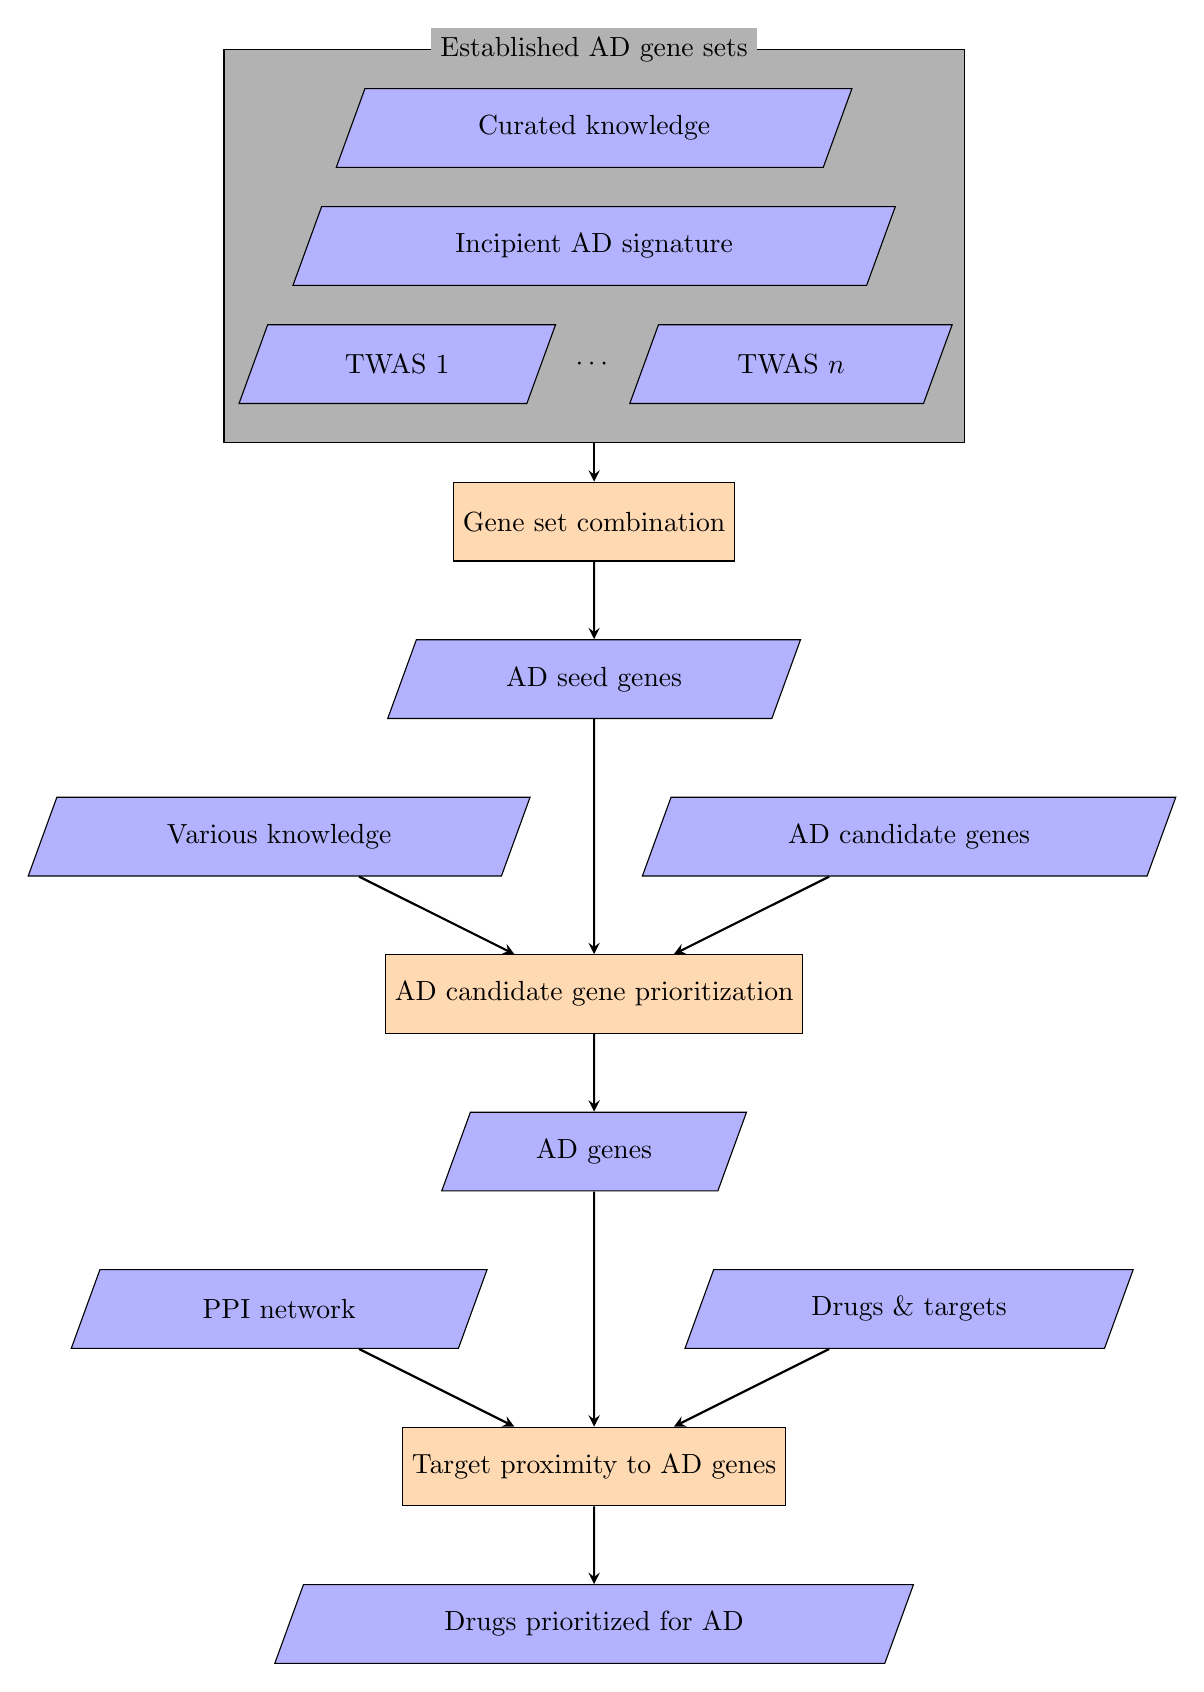
\begin{tikzpicture}[node distance=2cm]

% Established AD gene sets
\begin{scope}[node distance=1.5cm]
\node[io] (knowledge) at (0,0) {Curated knowledge};
\node[io, below of=knowledge] (incipient) at (0,0) {Incipient AD signature};
\node[below of=incipient] (a) {$\cdots$};
\node[io, left of=a, xshift=-1cm] (TWAS1) {TWAS $1$};
\node[io, right of=a, xshift=1cm] (TWASn) {TWAS $n$};
\end{scope}[node distance=1.5cm]

% gray rectangle for Established AD gene sets
% create coordinates to define rectangle
\begin{scope}[node distance=2.2cm]
\coordinate[left of=TWAS1] (b);
\coordinate[right of=TWASn] (c);
\end{scope}
\begin{scope}[node distance=1.00cm]
\node[above of=knowledge, fill=black!30] (d) {Established AD gene sets};
\coordinate[below of=TWAS1] (e);
\end{scope}
% draw box itself
\begin{pgfonlayer}{background}
\filldraw[fill=black!30] (b|-e) rectangle (c|-d);
\end{pgfonlayer}

% AD seed genes
\node[process, below of=a] (union) {Gene set combination};
\draw[arrow] (a|-e) -- (union);
\node[io, below of=union] (ADseed) {AD seed genes};
\draw[arrow] (union) -- (ADseed);

% AD candidate gene prioritization
\node[io, below of=ADseed, xshift=-4cm] (various) {Various knowledge};
\node[io, below of=ADseed, xshift=4cm] (candidate) {AD candidate genes};
\node[process, below of=ADseed, yshift=-2cm] (prioritize) {AD candidate gene prioritization};
\draw[arrow] (candidate) -- (prioritize);
\draw[arrow] (various) -- (prioritize);
\draw[arrow] (ADseed) -- (prioritize);
\node[io, below of=prioritize] (ADgenes) {AD genes};
\draw[arrow] (prioritize) -- (ADgenes);

% Proximity
\node[process, below of=ADgenes, yshift=-2cm] (proximity) {Target proximity to AD genes};
\draw[arrow] (ADgenes) -- (proximity);
\node[io, below of=ADgenes, xshift=-4cm] (PPI) {PPI network};
\draw[arrow] (PPI) -- (proximity);
\node[io, below of=ADgenes, xshift=4cm] (drugs) {Drugs \& targets};
\draw[arrow] (drugs) -- (proximity);
\node[io, below of=proximity] (ADdrugs) {Drugs prioritized for AD};
\draw[arrow] (proximity) -- (ADdrugs);

\end{tikzpicture}
\end{document}

